%----------------------------------------------------------------------------------------
%	PACKAGES AND THEMES
%----------------------------------------------------------------------------------------
\documentclass[aspectratio=169,xcolor=dvipsnames]{beamer}
\usetheme{Simple}

\usepackage{hyperref}
\usepackage{graphicx} % Allows including images
\usepackage{booktabs} % Allows the use of \toprule, \midrule and \bottomrule in tables
\usepackage{caption}
\usepackage[ruled,vlined]{algorithm2e}
\usepackage{ragged2e}
\usepackage{amsmath} % Para las expresiones matemáticas
\usepackage{amssymb} % Para los símbolos matemáticos


%----------------------------------------------------------------------------------------
%	TITLE PAGE
%----------------------------------------------------------------------------------------

% The title
\title[short title]{Optimización Multiobjetivo del Parámetro de Regularización en Imágenes Fotoacústicas}
%\subtitle{Subtitle}

\author[Pin-Yen] {Maximiliano Galindo}
\institute[UNAM] % Your institution may be shorthand to save space
{
    % Your institution for the title page
    Maestría en Ciencia e Ingeniería de la Computación  \\
    Universidad Nacional Autónoma de México
    \vskip 3pt
    \textbf{Supervisores:} \\
    Dr. Luis Agustín Alvarez-Icaza Longoria \\
    Dr. Roberto Giovanni Ramírez Chavarría \\
}
\date{29 de Noviembre del 2024} % Date, can be changed to a custom date


%----------------------------------------------------------------------------------------
%	PRESENTATION SLIDES
%----------------------------------------------------------------------------------------

\begin{document}

\begin{frame}
    % Print the title page as the first slide
    \titlepage
\end{frame}

\begin{frame}{Contenido}
    % Throughout your presentation, if you choose to use \section{} and \subsection{} commands, these will automatically be printed on this slide as an overview of your presentation
    \tableofcontents
\end{frame}

%------------------------------------------------
\section{Introducción}
%------------------------------------------------

\begin{frame}{Efecto Fotoacústico}
    \begin{columns}
        \begin{column}{0.5\textwidth}
            \begin{itemize}
                \item Las imágenes fotoacústicas combinan óptica y ultrasonido para aplicaciones biomédicas.
                \item Técnica no invasiva útil para evaluar tejidos arteriales y estudiar procesos celulares.
            \end{itemize}
        \end{column}
        \begin{column}{0.5\textwidth}
            \centering
            \includegraphics[width=\textwidth]{img/effect.pdf} % Reemplaza con la ruta a tu imagen
            \captionof{figure}{Efecto fotoacústico}
        \end{column}
    \end{columns}
\end{frame}

%------------------------------------------------

\begin{frame}{Efecto Fotoacústico}
    La ecuación que describe el efecto fotoacústico es:

    \begin{equation}
        \frac{\partial^2 p(z, t)}{\partial z^2} - \frac{1}{c_0^2} \frac{\partial^2 p(z, t)}{\partial t^2} + \tau \frac{\partial^3 p(z, t)}{\partial t \partial z^2} = -\frac{\beta}{C_p} \frac{\partial H(z, t)}{\partial t}.
    \end{equation}
    \begin{block}{Donde}
        \begin{itemize}
            \item $p(z, t)$ es la presión local a profundidad $z$ y tiempo $t$. 
            \item $c_0$ es la velocidad del sonido.
            \item $\tau$ es el tiempo de relajación.
            \item $\beta$ es el coeficiente de expanción térmica. 
            \item $C_p$ es el calor específico a presión constante. 
            \item $H(z, t) = R(z)i(t)$ es el producto de la absorción fraccional de energía $R(z)$ a profundidad $z$ y el perfil temporal de iluminación $i(t)$.
        \end{itemize}
    \end{block}
\end{frame}

    % \begin{block}{Block}
    %     Sample text
    % \end{block}

    % \begin{alertblock}{Alertblock}
    %     Sample text in red box
    % \end{alertblock}

    % \begin{examples}
    %     Sample text in green box. The title of the block is ``Examples".
    % \end{examples}

%------------------------------------------------
\section{Problema}
\begin{frame}{Problema}
    \begin{columns}[c] % The "c" option specifies centered vertical alignment while the "t" option is used for top vertical alignment

        \column{.5\textwidth} % Left column and width
        \begin{equation}
            \begin{gathered}
                \left[\nabla^2-\frac{1}{c^2} \frac{\partial^2}{\partial t^2}\right] P(\mathbf{x}, t)=0, \quad t \geq 0 \\ 
                P\left(\mathbf{x}^{\prime}, 0\right)=f\left(\mathbf{x}^{\prime}\right),\left.\quad \frac{\partial P}{\partial t}\right|_{t=0}=0 \\ 
                P\left(\mathbf{x}_S, t\right)=g\left(\mathbf{x}_S, t\right) \text { para } \mathbf{x}_S \in S, t \geq 0 .
            \end{gathered}
        \end{equation}

        \column{.5\textwidth} % Right column and width
        \centering
        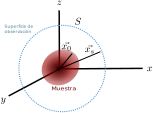
\includegraphics[width=\textwidth]{img/super.pdf} % Reemplaza con la ruta a tu imagen
        \captionof{figure}{Problema inverso en la reconstrucción fotoacústica.}

    \end{columns}
\end{frame}

%------------------------------------------------
\section{Enfoque de Modelo en Espacio de Estados Lineal}
%------------------------------------------------

\begin{frame}{Modelo en Espacio de Estados Lineal}
    Podemos modelar el problema como un modelo en espacio de estados lineal \cite{Lang}:

    \begin{equation}
        \begin{aligned}
            \mathbf{x}_{k+1} &= A \mathbf{x}_k + B \mathbf{u}_k \\
            \mathbf{y}_k &= C^{T} \mathbf{x}_k + \mathbf{w}_k
        \end{aligned}
    \end{equation}

    Con este enfoque, podemos encontrar la siguiente conexion lienal entre nuestras mediciones $\mathbf{y}$ y un vecotr $\mathbf{d}$ que contiene el perfil de absorción de nuestra muestra:
    
        \begin{equation} \label{eq:problem}
            \mathbf{y} = \mathbf{H} \mathbf{d} + \mathbf{w}
        \end{equation} 

\end{frame}


    % \begin{table}
    %     \begin{tabular}{l l l}
    %         \toprule
    %         \textbf{Treatments} & \textbf{Response 1} & \textbf{Response 2} \\
    %         \midrule
    %         Treatment 1         & 0.0003262           & 0.562               \\
    %         Treatment 2         & 0.0015681           & 0.910               \\
    %         Treatment 3         & 0.0009271           & 0.296               \\
    %         \bottomrule
    %     \end{tabular}
    %     \caption{Table caption}
    % \end{table}
%------------------------------------------------

%------------------------------------------------
\section{Regularización}
%-------------------------------------------------
\begin{frame}{Regularización}
    Debido a la naturaleza del problema, es necesario considerar metodos de regularización para solucionar la ecuación \ref{eq:problem}. Se propone el uso de la regularización de Tikhonov, la cual se define como:
    
    \begin{equation}
        \hat{\mathbf{d}} = \arg \min _{\mathbf{d}}\left\{\|\mathbf{y}-\mathbf{H} \mathbf{d}\|_{2}^{2}+\lambda\|\mathbf{d}\|_{2}^{2}\right\}
    \end{equation}

    \begin{block}{Donde}
        \begin{itemize}
            \item $\mathbf{d}$ es el vector de que queremos estimar.
            \item $\mathbf{H}$ es la matriz obtenida a partir de datos experimentales.
            \item $\lambda$ es el parámetro de regularización.
        \end{itemize}
    \end{block}
\end{frame}

%------------------------------------------------

\begin{frame}{Método de la Curva L}
    \begin{columns}
        \column{.5\textwidth}
        El método de la curva L es una técnica para seleccionar el parámetro de regularización $\lambda$ de manera automática. Se basa en graficar la norma del residuo contra la norma de regularización en escala logarítmica. El vértice de la curva representa el mejor compromiso entre ambos criterios.

        \column{.5\textwidth}
        \centering
        \includegraphics[width=\textwidth]{img/L_curve.png} % Reemplaza con la ruta a tu imagen
        \captionof{figure}{Método de la curva L.}
    \end{columns}
\end{frame}

%------------------------------------------------
\begin{frame}{Limitaciones de la Curva L}
    \begin{alertblock}{Limitaciones}
        \begin{itemize}
            \item Puede ser computacionalmente costosa en problemas de alta dimensionalidad, debido a la necesidad de resolver el sistema para múltiples valores de \(\lambda\).
            \item Es sensible al ruido y a la condición numérica de la matriz \(\mathbf{H}\), lo que puede generar resultados menos robustos.
            \item Requiere una búsqueda exhaustiva para identificar el vértice de la curva, aumentando el tiempo de cálculo en problemas grandes.
            \item No explora soluciones alternativas o trade-offs explícitos, ya que se enfoca en una única solución óptima.
            \item No considera explícitamente la naturaleza multiobjetivo del problema (e.g., fidelidad, regularización, y restricciones físicas como positividad).
        \end{itemize}
    \end{alertblock}
\end{frame}


%------------------------------------------------
\section{Optimización Multiobjetivo}
%------------------------------------------------

%------------------------------------------------
\begin{frame}{Optimización Multiobjetivo}
   La optimización multiobjetivo permite encontrar soluciones óptimas que equilibran múltiples objetivos en conflicto. En el contexto de la regularización de Tikhonov, los objetivos considerados son:
    \begin{block}{Objetivos}
        \begin{itemize}
            \item Minimizar el error de ajuste: \(||\mathbf{y} - \mathbf{H} \mathbf{d}||^2_2\).
            \item Minimizar la norma de la solución (regularización): \(||\mathbf{d}||^2_2\).
            \item Minimizar la penalización por valores negativos en \(\mathbf{d}\), asegurando soluciones físicamente significativas.
        \end{itemize}
    \end{block}
\end{frame}

%------------------------------------------------

\begin{frame}{Ventajas de la Optimización Multiobjetivo}
    \begin{block}{Ventajas}
        \begin{itemize}
            \item Permite explorar el espacio de soluciones y encontrar compromisos entre los objetivos definidos.
            \item Proporciona un conjunto de soluciones (frente de Pareto) que representan diferentes trade-offs entre los objetivos.
            \item Permite identificar soluciones que satisfacen restricciones físicas y son más robustas ante ruido y errores de medición.
            \item Proporciona información valiosa para la toma de decisiones y la selección de la solución más adecuada.
        \end{itemize}
    \end{block}
\end{frame}

%------------------------------------------------

\begin{frame}{NSGA-II}
    \begin{columns}[T] % Alineación superior para las columnas
        \column{.4\textwidth}
        \justifying % Para justificar el texto
        \textbf{NSGA-II (Non-dominated Sorting Genetic Algorithm II)} es un algoritmo evolutivo multiobjetivo que permite encontrar soluciones óptimas en problemas de optimización multiobjetivo. Este algoritmo clasifica las soluciones en diferentes frentes no dominados basándose en el concepto de \textit{dominancia de Pareto}. Su principal ventaja es la capacidad de generar soluciones diversas y bien distribuidas a lo largo del frente de Pareto \cite{Deb}.
        \vspace{1em} % Espaciado entre texto y columna derecha

        \column{.55\textwidth}
        \scriptsize % Ajusta el tamaño del texto para que quepa en la diapositiva
        \begin{algorithm}[H]
            \caption{NSGA-II Algorithm}\label{alg:nsga2}
            Inicializar $P$, $n_{\text{generations}}$ \tcp*[h]{Población inicial} \\
            $\mathcal{N} = |P|$\;
            $P_t \gets P$\;
            $Q_t \gets \text{make\_new\_pop}(P_t)$\;
            \While{$t < n_{\text{generations}}$}{
                $R_t \gets P_t \cup Q_t$\;
                $\mathcal{F} \gets \text{fast\_non\_dominated\_sort}(R_t)$\;
                $P_{t+1} \gets \emptyset$, $i \gets 1$\;
                \While{$|P_{t+1}| + |\mathcal{F}_i| \leq \mathcal{N}$}{
                    \text{crowding\_distance\_assignment}$(\mathcal{F}_i)$\;
                    $P_{t+1} \gets P_{t+1} \cup \mathcal{F}_i$\;
                    $i \gets i + 1$\;
                }
                %\EndWhile
                \text{Sort}$(\mathcal{F}_i, \prec_n)$ \tcp*[h]{Orden descendente usando $\prec_n$}\;
                $P_{t+1} \gets P_{t+1} \cup \mathcal{F}_i[1:(\mathcal{N} - |P_{t+1}|)]$\;
                $Q_{t+1} \gets \text{make\_new\_pop}(P_{t+1})$\;
                $t \gets t + 1$\;
            }
        \end{algorithm}
    \end{columns}
\end{frame}

%------------------------------------------------
\begin{frame}{MOEA/D}
    \begin{columns}[T]
        \column{.45\textwidth}
        \justifying
        \textbf{MOEA/D (Multiobjective Evolutionary Algorithm based on Decomposition)} descompone el problema multiobjetivo en múltiples subproblemas escalares. Cada subproblema se resuelve utilizando información de sus vecinos, logrando una mejor representación en el frente de Pareto.

        % \vspace{0.5em}
        % \textbf{Características principales:}
        % \begin{itemize}
        %     \item Divide el problema en subproblemas utilizando métodos como Tchebycheff o pesos ponderados.
        %     \item Promueve la cooperación entre soluciones vecinas.
        %     \item Genera frentes más uniformes y equilibrados.
        % \end{itemize}

        \column{.55\textwidth}
        \scriptsize
        \begin{algorithm}[H]
            \caption{MOEA/D Algorithm}\label{alg:moead}
            \textbf{Entrada:} Población inicial $P$, vectores de peso $\lambda$, vecindario $T$\;
            \textbf{Salida:} Soluciones no dominadas\;
            Inicializar población y vecindarios\;
            \For{$t = 1$ \KwTo $n_{\text{generations}}$}{
                \ForEach{subproblema $i$}{
                    Seleccionar vecinos $B(i)$\;
                    Generar nueva solución $y$ mediante cruce y mutación\;
                    Evaluar $y$ y actualizar población\;
                    \ForEach{$j \in B(i)$}{
                        \If{$g(y, \lambda_j) < g(P_j, \lambda_j)$}{
                            Reemplazar $P_j$ con $y$\;
                        }
                    }
                }
            }
            Retornar soluciones no dominadas\;
        \end{algorithm}
    \end{columns}
\end{frame}

%------------------------------------------------
\section{Resultados}
%------------------------------------------------

\begin{frame}{Frente de Pareto NSGA-II}
    \begin{columns}
        \column{.45\textwidth}
        \justifying
        Se aplicó el algoritmo NSGA-II para estimar el parametro de regularización $\lambda$ para la reconstrucción del perfil de absorción donde el ruido fue modelado como una distribución normal $\mathcal{N}(0, 0.1)$. Se obtuvo un frente de Pareto que muestra diferentes trade-offs entre el error de ajuste y la regularización.

        \column{.5\textwidth}
        \centering
        \includegraphics[width=\textwidth]{img/pareto_front_nsga2.png} \label{fig:pareto_nsga2} 
        \captionof{figure}{Representación de un frente de Pareto.}
    \end{columns}
\end{frame}

%------------------------------------------------

\begin{frame}{Frente de Pareto NSGA-II}
    \begin{columns}
        \column{.45\textwidth}
        \justifying
        Podemos agrupar las soluciones del frente de Pareto en diferentes categorías según su desempeño en los objetivos definidos.
        \column{.5\textwidth}
        \centering
        \includegraphics[width=\textwidth]{img/pareto_clustering_nsga2.png} \label{fig:pareto_clustering_nsga2}
        \captionof{figure}{Representación de un frente de Pareto.}
    \end{columns}
\end{frame}

%------------------------------------------------

\begin{frame}{Frente de Pareto MOEA/D}
    \begin{columns}
        \column{.45\textwidth}
        \justifying
        Se aplicó el algoritmo MOEA/D para estimar el parametro de regularización $\lambda$ para la reconstrucción del perfil de absorción donde el ruido fue modelado como una distribución normal $\mathcal{N}(0, 0.1)$. Se obtuvo un frente de Pareto que muestra diferentes trade-offs entre el error de ajuste y la regularización.

        \column{.5\textwidth}
        \centering
        \includegraphics[width=\textwidth]{img/pareto_front_moead.png} \label{fig:pareto_moead}
        \captionof{figure}{Representación de un frente de Pareto.}
    \end{columns}
\end{frame}

%------------------------------------------------

\begin{frame}{Frente de Pareto MOEA/D}
    \begin{columns}
        \column{.45\textwidth}
        \justifying
        Podemos agrupar las soluciones del frente de Pareto en diferentes categorías según su desempeño en los objetivos definidos.
        \column{.5\textwidth}
        \centering
        \includegraphics[width=\textwidth]{img/pareto_clustering_moead.png} % Reemplaza con la ruta a tu imagen
        \captionof{figure}{Representación de un frente de Pareto.}
    \end{columns}
\end{frame}

%------------------------------------------------
\begin{frame}{Correlación entre los Objetivos}
    Se evaluó la correlación entre los objetivos definidos en el problema de optimización multiobjetivo, así como las proyecciones de las soluciones en el espacio de objetivos generadas por NSGA-II y MOEA/D.
    
    \begin{columns}
        \column{.33\textwidth}
        \centering
        \includegraphics[width=\textwidth]{img/correlation_matrix.png} % Reemplaza con la ruta a tu imagen
        \captionof{figure}{Matriz de correlación entre los objetivos.}
        
        \column{.33\textwidth}
        \centering
        \includegraphics[width=\textwidth]{img/pareto_projection_nsga2.png} % Reemplaza con la ruta a tu imagen
        \captionof{figure}{Proyecciones de las soluciones en el espacio de objetivos (NSGA-II).}
        
        \column{.33\textwidth}
        \centering
        \includegraphics[width=\textwidth]{img/pareto_projection_moead.png} % Reemplaza con la ruta a tu imagen
        \captionof{figure}{Proyecciones de las soluciones en el espacio de objetivos (MOEA/D).}
    \end{columns}
    
\end{frame}

%------------------------------------------------
\begin{frame}{Reconstrucción del Perfil de Absorción}
    Las soluciones seleccionadas en los frentes de Pareto \ref{fig:pareto_nsga2} y \ref{fig:pareto_moead} fueron seleccionadas en base a su desempeño en los objetivos definidos utilizando un sistema de puntacion ponderado de 80 $\%$ para el error de ajuste, 10 $\%$ para la regularización y 10 $\%$ para la penalización por valores negativos.

    \begin{columns}
        \column{.5\textwidth}
        \centering
        \includegraphics[width=\textwidth]{img/reconstruction_profiles_nsga2.png} % Reemplaza con la ruta a tu imagen
        \captionof{figure}{Reconstrucción del perfil de absorción con NSGA-II.}
        \column{.5\textwidth}
        \centering
        \includegraphics[width=\textwidth]{img/reconstruction_profiles_moead.png} % Reemplaza con la ruta a tu imagen
        \captionof{figure}{Reconstrucción del perfil de absorción con MOEA/D.}
    \end{columns}
\end{frame}

%------------------------------------------------
\begin{frame}{Comparacion entre NSGA-II, MOEA/D y la Curva L}

    \begin{table}[h]
        \centering
        \begin{tabular}{lccc}
            \toprule
            \textbf{Método} & \textbf{Fidelidad (\( f_1 \))} & \textbf{Regularización (\( f_2 \))} & \textbf{Negatividad (\( f_3 \))} \\
            \midrule
            NSGA-II (mejor solución) & 0.000 & 1.000 & 0.000 \\
            MOEA/D (mejor solución) & 0.000 & 1.000 & 0.347 \\
            Curva L & 0.00063 & 0.0071 & 0.0001 \\
            \bottomrule
        \end{tabular}
        \caption{Comparación de las métricas entre NSGA-II, MOEA/D y la curva L. Los valores están normalizados para permitir una evaluación directa.}
        \label{tab:comparison_algorithms}
    \end{table}
    
\end{frame}

%------------------------------------------------
\begin{frame}{Impacto del Ruido en el RMSE}
    Con la misma ponderación, se evaluó el impacto del ruido en el RMSE de las soluciones generadas mediante NSGA-II y MOEA/D, comparándolas con las obtenidas mediante la Curva L y el método de mínimos cuadrados.
    
    \begin{columns}
        \column{.5\textwidth}
        \centering
        \includegraphics[width=\textwidth]{img/impact_noise_on_rmse_nsga2.png} % Reemplaza con la ruta a tu imagen
        \captionof{figure}{Impacto del ruido en el RMSE con NSGA-II.}
        \column{.5\textwidth}
        \centering
        \includegraphics[width=\textwidth]{img/impact_noise_on_rmse_moead.png} % Reemplaza con la ruta a tu imagen
        \captionof{figure}{Impacto del ruido en el RMSE con MOEA/D.}
    \end{columns}
\end{frame}




%------------------------------------------------
\section{Trabajo por hacer}
%------------------------------------------------
\begin{frame}{Trabajo por hacer}
    \begin{block}{To Do}
        \begin{itemize}
            \item Extender la reconstrucción a dominios 2D para evaluar la escalabilidad de los algoritmos.
            \item Optimizar los hiperparámetros de los algoritmos multiobjetivo para mejorar su desempeño en exploración y convergencia.
            \item Analizar más a fondo las interacciones entre objetivos para guiar el diseño de algoritmos específicos para aplicaciones biomédicas.
        \end{itemize}
    \end{block}
\end{frame}
    
        
    
% Este enfoque genera un conjunto de soluciones (frente de Pareto) que representan compromisos entre los objetivos definidos.
        
% \column{.5\textwidth}
% \centering
% \includegraphics[width=\textwidth]{img/multiobj.pdf} % Reemplaza con la ruta a tu imagen
% \captionof{figure}{Representación de un frente de Pareto.}
% \end{columns}

\begin{frame}{Referencias}
    % Beamer does not support BibTeX so references must be inserted manually as below
    \footnotesize{
        \begin{thebibliography}{99}
            \bibitem[Deb et al., 2002]{Deb} K. Deb, A. Pratap, S. Agarwal, and T. Meyarivan (2002)
            \newblock A fast and elitist multiobjective genetic algorithm: NSGA-II
            \newblock \emph{IEEE Transactions on Evolutionary Computation}, 6(2), 182–197. DOI: \url{https://doi.org/10.1109/4235.996017}.
            
            \bibitem[Zhang and Li, 2007]{Zhang} Q. Zhang and H. Li (2007)
            \newblock MOEA/D: A multiobjective evolutionary algorithm based on decomposition
            \newblock \emph{IEEE Transactions on Evolutionary Computation}, 11(6), 712–731. DOI: \url{https://doi.org/10.1109/TEVC.2007.892759}.
            
            \bibitem[Lang et al., 2019]{Lang} Oliver Lang, Péter Kovács, Christian Motz, Mario Huemer, Thomas Berer, and Peter Burgholzer (2019)
            \newblock A linear state space model for photoacoustic imaging in an acoustic attenuating media
            \newblock \emph{Inverse Problems}, 35(1), 015003. DOI: \url{https://doi.org/10.1088/1361-6420/aaea2c}.
        \end{thebibliography}        
    }
\end{frame}

%------------------------------------------------

\begin{frame}
    \Huge{\centerline{Gracias.}}
\end{frame}

%----------------------------------------------------------------------------------------

\end{document}